

\begin{figure}[h]
    \centering
    % \begin{minipage}[t]{0.49\textwidth}
    %     \centering
    %     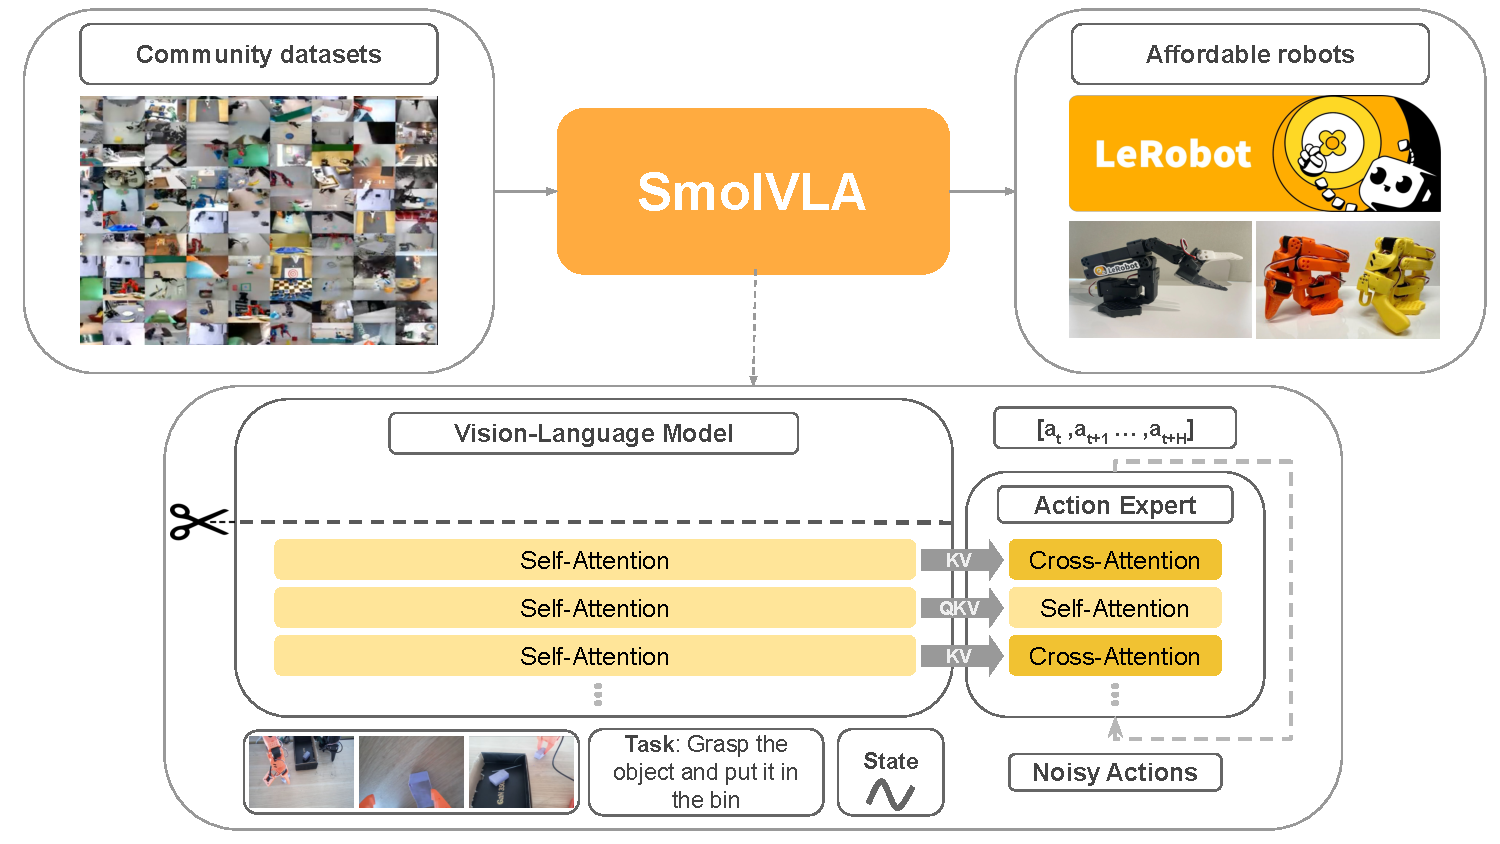
\includegraphics[width=\textwidth]{figures/SmolVLA.pdf}
    %     \caption{\footnotesize \textbf{Summary of the work.}}
    %     \label{fig:teaser}
    % \end{minipage}
    % \hfill
    \begin{minipage}[t]{1\textwidth}
        \centering
        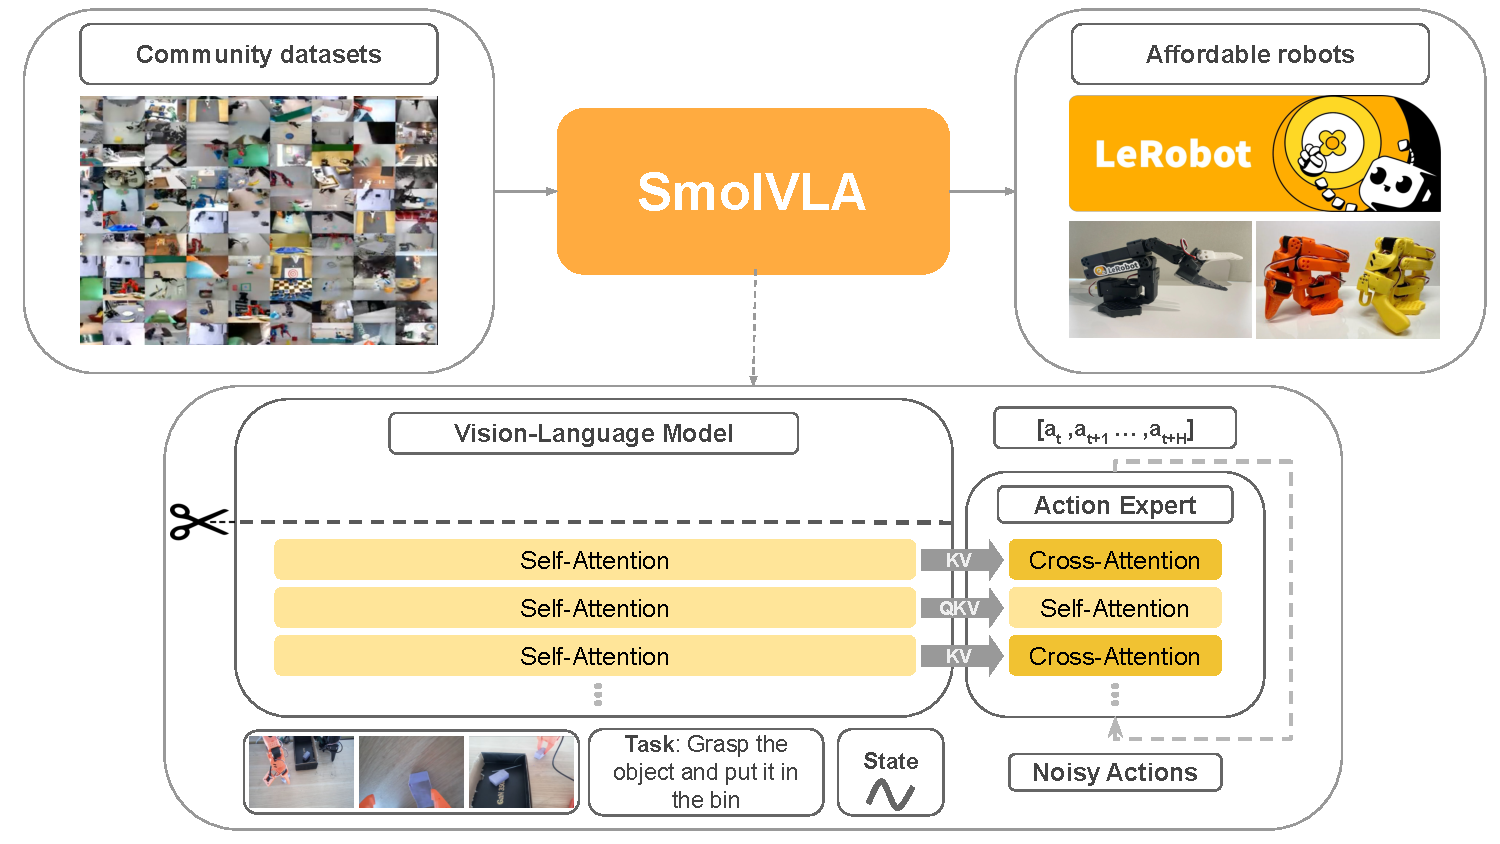
\includegraphics[width=0.88\textwidth]{figures/SmolVLA.pdf}
        \caption{\footnotesize \textbf{SmolVLA.} SmolVLA consists of a compact pretrained vision-language model, discarding the last $L-N$ layers (scissors icon). The remaining layers embed three inputs: (i) language instruction, (ii) RGB image(s), and (iii) robot sensorimotor state. Their merged tokens feed an Action Expert of alternating cross-attention (gold) and self-attention (light yellow) blocks, trained with flow matching to output $n$ low-level actions chunk $a_t, \dots, a_{t+n}$. SmolVLA is pretrained on public community datasets and evaluated on low-cost robots.
        % Key differences with respect to $\pi_0$: (1) Interleaved cross/self-attention blocks, (2) First-N VLM layers only used, (3) State inputs fed to VLM, (4) Larger action expert, (5) Causal attention on actions, (6) Smaller policy.
        }
        \label{fig:arch}
    \end{minipage}
    \vspace{-0.6cm}
\end{figure}



\section{Introduction}

In recent years, the field has shifted towards the development of \emph{foundation} models, generalist models capable of performing a wide range of tasks.
A prominent example of this trend are large language models (LLMs), which have demonstrated performance comparable to the average human in understanding and generating natural language, reasoning over complex topics, and anchoring in knowledge~\citep{GPT3,GPT4,Llama3,Gemini,Mistral7B}. 
The success of text-based models has thus been extended to other modalities, sparking interest towards multi-modal vision-language (VLMs)~\citep{alayrac2022flamingo,PaLI-3,kosmoshuang2023language,LLaVA-1.5,chen2024internvl25,shukor2023unival} and audio-language models (ALMs)~\citep{defossez2024moshi,das2024speechverse,borsos2023audiolm}. 
While complementary in terms of modalities, such advances in developing multi-modal foundation models stem from \emph{(i)} the adoption of scalable architectures, such as the Transformer~\citep{vaswani2017attention} and \emph{(ii)} internet-scale training datasets.

Despite their remarkable achievements in the digital world, real-world application of foundation models--particularly in robotics--remains limited. 
In particular, robotic policies~\citep{zhao2023learningact,chi2024diffusionpolicy,lee2024behavior,Hansen2022tdmpc} still face challenges in generalizing across object types, positions, environments, and tasks~\citep{xie2024decomposing,ebert2021bridge}. 
Robots should be able to adapt to new surroundings and new objects, which requires robust skills and common sense understanding of the world. Yet, the progress in this direction seems to be often limited by the availability of high-quality and diverse data.
%A key barrier to scalability in robotics is the scarcity of high-quality, diverse data.

To address this limitation, a growing body of work has begun exploring robotics foundation models in the form of vision-language-action (VLA) models~\citep{team2024octo,o2024openrtx,brohan2023rt2,kimopenvla,black2024pi_0,bjorck2025gr00t,li2024vision,huang2024embodied}.
VLAs are designed to incorporate abstract reasoning, world knowledge, and decision-making skills embedded in pretrained large language and vision-language models. 
These models take multimodal inputs--such as visual observations and natural language instructions--and predict the corresponding robotic actions. 
Early results suggest promising gains in generalization capabilities \citep{black2024pi_0,brohan2023rt2}.

VLA models remain in an early stage of development and are not yet as mature or widely adopted as LLMs and VLMs. Much of the impactful VLA progress remains proprietary, with many models sharing only weights while withholding full training details and essential methodological components.
While effective in tackling academic benchmarks, we argue achieving human-level capabilities in robotics requires a stronger commitment to open-source efforts. In particular, transparent, reproducible open-source models and training recipes are crucial for accelerating progress and fostering broader participation within the robotics research community.
We advocate for the development of affordable, efficient models that are accessible to a broader community. 
While encouraging efforts like OpenVLA \citep{kimopenvla} and RT-2-X \citep{o2024openrtx} demonstrate the feasibility of open VLA systems, they remain large, resource-intensive, and dependent on costly robotic platforms, hindering accessibility.

In this work, we introduce \ours, an open-source initiative featuring a compact yet capable VLA model, released alongside reproducible and efficient training and inference recipes.
% I kinda like explicitly listing contributions when going through papers
Our contributions are as follows:
\begin{itemize}
    \item \textbf{Lightweight architecture.} We present \ours, a compact and efficient vision-language agent optimized for training on consumer-grade GPUs and deployment on CPUs. Key design choices include: \emph{(i)} skipping layers in the VLM, \emph{(ii)} using a minimal number of visual tokens \emph{(iii)} leveraging small pretrained VLMs, and \emph{(iv)} interleaving self-attention layers with lighter cross-attention layers.
    \item \textbf{Pretraining on community-driven datasets.} \ours is trained end-to-end on fewer than 30k episodes drawn entirely from publicly available, community-contributed datasets, demonstrating strong performance while using an order of magnitude less data than prior art.
    \item \textbf{Asynchronous inference.} We introduce an optimized asynchronous inference stack that decouples action execution from observation processing and action prediction, reducing latency and enabling fast, resource-efficient inference.
\end{itemize}


% \ours is designed to be trainable on consumer-grade GPUs and deployable directly on CPUs.
% \ours is trained entirely on publicly available, community-contributed datasets, incorporated both in pretraining and post-training phases.
% In keeping with~\citet{zhou2024transfusion,black2024pi_0}, \ours combines transformers with flow matching, and is optimized for speed and efficiency during both training and inference.
% In particular, key design choices include: \emph{(i)} skipping layers in the VLM, \emph{(ii)} interleaving self-attention layers with lighter cross-attention layers, \emph{(iii)} using a minimal number of visual tokens, and \emph{(iv)} leveraging small pretrained VLMs.

% Pretraining is performed on a collection of community datasets comprising fewer than 30k episodes--an order of magnitude smaller than prior art.

% To support faster reaction time during inference, we also propose an asynchronous inference stack that decouples action execution from observation processing and action prediction.

We evaluate \ours on both simulated environments and real-world settings on multiple tasks. Interestingly, although significantly smaller, \ours matches or surpasses the performance of much larger VLA models.

